\chapter{Literature Review}

Except the initial work done by Axelrod, there are many other papers that have tried
to tangle the proble of PD and make their conclusions on cooperational debaviour in
both theorytical and ral life behavior. In this chapter we review some of this work
done in the IPD competitions, in spatial and evolutionary game theory.

\section{The Prisoner's Dilemma}
The PD was originally formulated by Merril M. Flood and Melvin Dresher,
who were working on the Flood-Desher Experiment at the RAND cooperation in 1950.
Later in 1950, the mathematician Albert W. Tucker presented the first formal
representation of the PD, titled  A Two-Person Dilemma in a seminar at
Stanford University\parencite{Gass005}.

A description of the PD, found in \parencite{Li2011} is as follows :
There are two players that simultaneously have to decide to whether Cooperate(C)
or Defect (D) with each other, without exchanging informations.

\begin{itemize}
  \item If both players choose to cooperate they will both receive a reward (R)
  \item If a player defects and the other cooperates then the defector receives
  a temptation payoff (T) and the cooperator a sucker payoff (S)
  \item If both players defect they will both receive a penalty (P)
\end{itemize}

Fig. 1 illustrates the payoffs matrix.~\ref{fig:pd_payoff}.

\begin{figure}[h!]
\centering
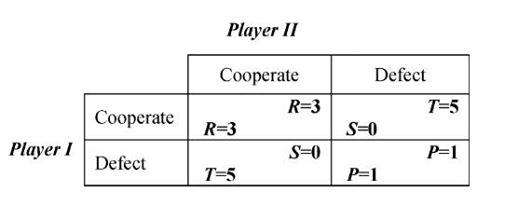
\includegraphics[scale=0.45]{pd_payoff.jpg}
\caption{Prisoner's Dilemma Payoff Matrix.\parencite{Li2011}}
\label{fig:pd_payoff}
\end{figure}

Taking into acount the assumptions that both players are both rational human beings and
that there is no way of communication between them,it can be shown that in the standar
form of the PD a pure Nash Equilibrium existswhen both players defect.
So the outcome of any one round game will be Defection.

The Prisoner’s Dilemma can also be studied for any given number of interations (IPD)
, where players play each other repeatedly. An extra condition for the payoffs
in the IPD are : T \(>\) R \(>\) P \(>\) S and R \(>\) 1/2(T+S).

\section{Tournaments}

In 1980-81, Robert Axelrod conducted a computer tournement where different
strategies for the Iterated Prisoner's Dilemma(IPD) clashed and a winner was annouched.
With 13 and 62 strategies respectively both tournaments shared the same topology
(round robin) and the same winner, which was Tit for Tat.
Moreover, Axelrod proved that cooperative behaviour emerging
depends on the probability of two players meeting  again.


Axelrod began an age of Game Theory and computer programming.
After his work various research was conducted trying to sight some light on the
cooperation evolution in IPD.

\section{Spatial Structure Tournaments}

Nowak and May, 1992, conducted their own experiment but this
time using a different topology that Axelrod. Instead of all the players playing
each other, this time the players would be represented in a lattice and they would
only play their neighbors.

After Nowak many other reserachers experimented with the spatial structure and
most of them used a 2D sqare lattice. Differences can be found between using
the PD or the IPD and whether there was evolution in their tournaments.

\section{Evolution and Moran process}
\lipsum[1-10]
